\documentclass[11pt,a4paper]{article}

\usepackage{main}
\usepackage{cours}

\renewcommand{\typedocument}{Cours}
\renewcommand{\classe}{3e}
\renewcommand{\titre}{Récapitulatif de chimie}

\begin{document}

\pagination

% ==================================================
\partie{Constitution de la matière}

Une \important{espèce chimique} est un ensemble d'entités chimiques identiques
(molécule, ion, atome).

\vspace*{-0.5em}

\souspartie{L'atome}

Un atome est constitué de 3 types de particules :
\begin{itemize}
    \item les \important{nucléons} : les \important{protons} (chargés
    \important{positivement}) et les \important{neutrons} (\important{sans charge})
    forment le noyau ;
    \item un nuage d'électrons : les \important{électrons} (chargés
    \important{négativement}) gravitent autour du noyau.
\end{itemize}

On note l'atome ${}^{A}_{Z}\mathrm{X}$ avec :
\begin{itemize}
    \item $\mathrm{X}$ : le symbole de l'élément ;
    \item $A$ : le nombre de nucléons ;
    \item $Z$ : le \important{numéro atomique}, égal au nombre de protons.
\end{itemize}

On en déduit $N = A - Z$, le nombre de neutrons.

Dans un atome, il y a autant d'électrons que de protons : l'atome est
électriquement neutre.

Cette notation se trouve dans le tableau périodique des éléments.

\textbf{Atomes à connaître :} Carbone (C), Hydrogène (H), Oxygène (O), Azote (N).

\vspace*{-0.5em}

\souspartie{La molécule}

Une \important{molécule} est un ensemble d'atomes reliés entre eux. La formule
chimique de la molécule indique quels atomes la forment, et combien.

\exemple{La molécule d'eau H\textsubscript{2}O est constituée de 2 atomes d'hydrogène et 1 atome d'oxygène.}

\textbf{Molécules à connaître :} dioxygène ($\mathrm{O_2}$), dihydrogène
($\mathrm{H_2}$), diazote ($\mathrm{N_2}$), eau ($\mathrm{H_2O}$), dioxyde de
carbone ($\mathrm{CO_2}$), méthane ($\mathrm{CH_4}$), protoxyde d'azote
($\mathrm{N_2O}$).

\vspace*{-0.5em}

\souspartie{Les ions}

Les \important{ions} sont des molécules ou des atomes qui ont perdu ou gagné un
ou plusieurs électrons : ils sont chargés électriquement.
\begin{itemize}
    \item s'il a perdu un ou plusieurs électrons, il est chargé positivement, et
    sa formule chimique contient un $+$ (exemple : $\mathrm{Na^+}$, $\mathrm{Cu^{2+}}$) ;
    \item s'il a gagné un ou plusieurs électrons, il est chargé négativement, et
    sa formule chimique contient un $-$ (exemple : $\mathrm{Cl^-}$, $\mathrm{OH^-}$).
\end{itemize}

% ==================================================
\partie{Propriétés de la matière}

\vspace*{-0.5em}

\souspartie{États de la matière}

\noindent
\begin{minipage}[c]{0.55\linewidth}
La matière peut se présenter sous trois différents états : l'état liquide,
solide ou gazeux.

Lors d'une \important{transformation physique}, l'état de la matière est modifié,
mais l'espèce chimique reste la même. Le changement d'état se fait à une
température donnée. La masse est conservée, mais le volume change.
\end{minipage}%
\hfill
\begin{minipage}[c]{0.4\linewidth}
    \centering
    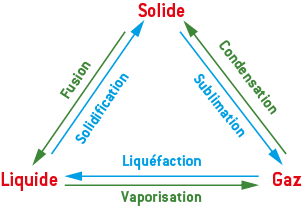
\includegraphics[width=4cm]{images/changements-etats.png}
\end{minipage}

\vspace*{-0.5em}

\souspartie{Mélanges}

Un \important{corps pur} est constitué d'une seule espèce chimique.

À l'inverse, dans un \important{mélange}, différentes espèces chimiques se mêlent.
Un mélange est dit \important{hétérogène} si on distingue les différentes espèces,
et \important{homogène} si on ne peut pas les distinguer.

Si deux liquides forment un mélange homogène, on dit qu'ils sont
\important{miscibles}.

Si un solide forme un mélange homogène dans l'eau, on dit qu'il est
\important{soluble}.

L'\important{air} est un mélange constitué d'environ 78\,\% de diazote (N\textsubscript{2}), 21\,\% de dioxygène (O\textsubscript{2}) et 1\,\% d'autres gaz.

\newpage

\vspace*{-0.5em}

\souspartie{Masse volumique}

La masse $m$ et le volume $V$ d'un objet sont deux grandeurs proportionnelles ;
on appelle le coefficient de proportionnalité la \important{masse volumique}
$\rho$.

\begin{center}
    \LARGE\important{$\rho = \dfrac{m}{V}$}
\end{center}

\begin{itemize}
    \item $\rho$ : la masse volumique, en \si{\kilogram/\cubic\metre} ;
    \item $m$ : la masse, en \si{\kilogram} ;
    \item $V$ : le volume, en \si{\cubic\metre}.
\end{itemize}

\vspace*{-0.5em}

L'unité principale est le \si{\kilogram/\cubic\metre}, mais il existe d'autres
unités comme le \si{\gram/\litre}, le \si{\kilogram/\litre} ou le
\si{\gram/\milli\litre}.

On peut identifier l'espèce chimique d'un objet à partir de sa masse volumique.

% ==================================================
\partie{Transformations chimiques}

\vspace*{-0.5em}

\souspartie{Acides et bases}

Une solution aqueuse contient des ions hydrogène $\mathrm{H^+}$ et des ions
hydroxyde $\mathrm{OH^-}$.

Selon l'ion majoritaire, on dit que la solution est \important{acide} ou
\important{basique}. Cela se détermine par le \important{pH}, une grandeur sans
unité, que l'on peut mesurer avec un pH-mètre ou du papier pH.
\begin{itemize}
    \item si le pH est inférieur à 7, la solution est acide (majorité d'ions
    $\mathrm{H^+}$) ;
    \item si le pH est égal à 7, la solution est neutre ;
    \item si le pH est supérieur à 7, la solution est basique (majorité d'ions
    $\mathrm{OH^-}$).
\end{itemize}

\vspace*{-0.5em}

\souspartie{Transformations chimiques}

Les différentes espèces chimiques (ions, atomes, molécules) peuvent réagir
ensemble lors d'une \important{transformation chimique}.

Une transformation chimique correspond à une redistribution des atomes : des
espèces chimiques disparaissent (les \important{réactifs}) et de nouvelles
espèces apparaissent (les \important{produits}). Il ne s'agit donc ni d'un
mélange ni d'une transformation physique.

\exemple{combustion du méthane : $\mathrm{CH_4} + 2\,\mathrm{O_2} \rightarrow
\mathrm{CO_2} + 2\,\mathrm{H_2O}$}

On peut résumer une transformation chimique par une \important{équation de
réaction}. Lors d'une transformation chimique, la masse se conserve.

Les transformations chimiques que l'on étudie sont :
\begin{itemize}
    \item les combustions ;
    \item les réactions acide-base ;
    \item les réactions acide-métaux.
\end{itemize}

\souspartie{Tests caractéristiques et protocoles expérimentaux}

\vspace*{-0.5em}

Les \important{tests caractéristiques} permettent d'identifier des espèces
chimiques.

\textbf{Protocole d'identification d'un ion :}
\begin{enumerate}
    \item verser un peu de la solution à tester dans un tube à essai ;
    \item à l'aide d'une pipette, ajouter quelques gouttes du réactif ;
    \item observer la formation et la couleur d'un éventuel précipité.
\end{enumerate}

\end{document}